\documentclass[border=5pt]{standalone}
\usepackage{tikz}
\usepackage{amsmath}
\usetikzlibrary{arrows.meta,calc,positioning,fit,backgrounds}
\definecolor{cpl}{RGB}{28,90,214}   % coupling blue
\definecolor{gh}{RGB}{110,110,110}  % ghost grey
\tikzset{
  bus/.style={circle, draw, line width=0.7pt, minimum size=15pt, inner sep=0pt, font=\footnotesize},
  ghost/.style={circle, draw=gh, line width=0.7pt, densely dotted, minimum size=15pt, inner sep=0pt, font=\footnotesize, text=gh},
  branch/.style={line width=0.75pt},
  stub/.style={gh, line width=0.75pt, densely dotted},
  halfl/.style={line width=0.75pt},
  zbox/.style={draw, fill=black!9, rounded corners=2pt, inner sep=3pt, font=\footnotesize},
  couple/.style={cpl, densely dotted, line width=0.9pt},
  cplab/.style={font=\scriptsize, text=cpl, inner sep=1.5pt},
  zone/.style={draw, dashed, rounded corners=7pt, line width=0.8pt, inner sep=0pt},
  zlab/.style={font=\scriptsize\itshape, text=black!55},
  gen/.style={circle, draw, line width=0.6pt, minimum size=11pt, inner sep=0pt, font=\scriptsize},
}

\begin{document}
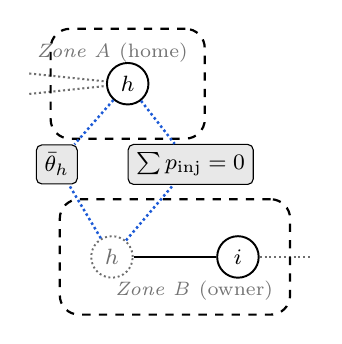
\begin{tikzpicture}
% ---------------- Zone A (top): home zone, real boundary bus h ----------------
\node[bus] (hA) at (1.1,2.2) {$h$};
\draw[stub] (-0.15,2.33) -- (hA);
\draw[stub] (-0.15,2.07) -- (hA);
\node[zone, fit=(hA), inner xsep=20pt, inner ysep=12pt] (zA) {};
\node[zlab, anchor=north east] at ([shift={(-3pt,-2pt)}]zA.north east) {Zone A \textup{(home)}};

% ---------------- Zone B (bottom): owner zone, owns the whole branch ----------------
\node[ghost] (hB) at (0.9,0.0) {$h$};
\node[bus]   (iB) at (2.5,0.0) {$i$};
\draw[branch] (hB) -- (iB);
\draw[stub]   (iB) -- (3.45,0.0);
\node[zone, fit=(hB)(iB), inner xsep=11pt, inner ysep=13pt] (zB) {};
\node[zlab, anchor=south east] at ([shift={(-3pt,2pt)}]zB.south east) {Zone B \textup{(owner)}};

% ---------------- consensus: state + injection ----------------
\node[zbox] (zth) at (0.2,1.175) {$\bar\theta_h$};
\node[zbox] (zinj) at (1.9,1.175) {$\textstyle\sum p_{\mathrm{inj}}=0$};
\draw[couple] (hA) -- (zth);
\draw[couple] (hB) -- (zth);
\draw[couple] (hA) -- (zinj);
\draw[couple] (hB) -- (zinj);
\end{tikzpicture}
\end{document}
